\chapter{Sử dụng PICKit 2 Programmer}
\tocless \section{Giới thiệu chung}
\begin{list}{--}{}
\item Giao tiếp qua cổng USB, không cần cài đặt Driver.
\item Hổ trợ các loại PIC: PIC10F, PIC12F5xx, PIC16F5xx, PIC12F6xx, PIC16F, PIC18F, PIC24, dsPIC30, dsPIC33, PIC32 với 8 bit, 16 bit, 32 bit và một số sản phẩm Serial Eprom của Microchip.
\end{list}
\tocless \section{Phần mềm giao tiếp với PICkit 2}
Sử dụng phần mềm PICKit 2 Programmer, các chức năng chính thường dùng trong phần mềm (giao diện trong \textit{hình ~\ref{Fig:PICKIT-2}}):
\begin{figure}[!h]
\begin{center}
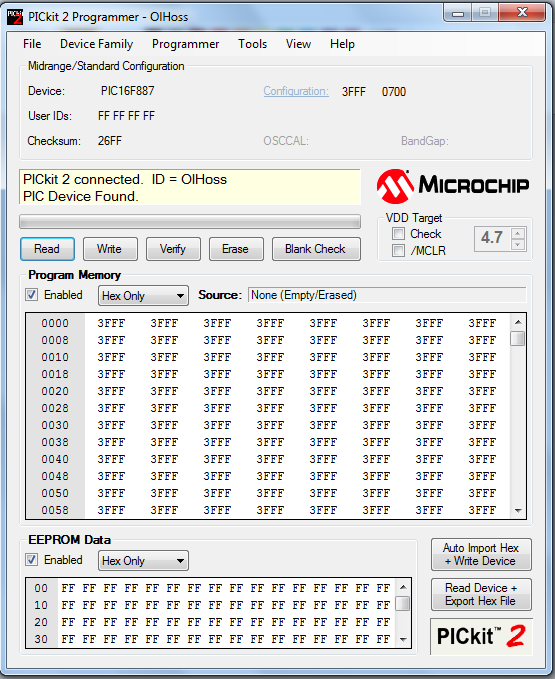
\includegraphics[scale=.5]{phu-luc/image/pickit-21}
\end{center}
\caption{Giao diện của phần mềm PICKit 2 Programmer}
\label{Fig:PICKIT-2}
\end{figure}
\begin{itemize}
\item Thẻ \verb|Tab|:
\begin{list}{--}{}
\item \verb|Import Hex|: Tải một file Hex vào bộ nhớ tạm.
\item \verb|Export Hex|: Xuất ra một file Hex có trong bộ nhớ tạm.
\end{list}
\item Thẻ \verb|Programmer|:
\begin{list}{--}{}
\item \verb|Read Device|: đọc nội dung chip như \verb|Program memory|, \verb|EEPROM data| đưa vào bộ nhớ tạm.
\item \verb|Write  Device|: nạp nội dung như \verb|Program  memory|, \verb|EEPROM data| đưa vào bộ nhớ tạm vào chip.
\item \verb|Verify|: so sánh nội dung của chip với nội dung trong bộ nhớ tạm.
\item \verb|Erase|: Xóa toàn bộ nội dung trong chip.
\end{list}
\item Thẻ \verb|Tools|:
\begin{list}{--}{}
\item \verb|Enable Code Protect|: khóa chương trình, chống sao chép.
\item \verb|Enable Data Protect|: khóa bộ nhớ \verb|EEPROM data| chống sao chép.
\item \verb|Fast programming|: nếu chọn chức năng này thì PICKit 2 sẽ nạp nhanh hơn, bình thường (chưa chọn) thì sẽ nạp chậm và độ tin cậy cao hơn.
\item \verb|Check Communication|: Kiểm tra giao tiếp giữa PC với PICkit 2 và ICSP giúp dò tìm chip.
\end{list}
\end{itemize}
\tocless \section{Nạp chương trình cho PIC}
Thực hiện theo các bước:
\begin{list}{--}{}
\item \textit{Bước 1}: Vào thẻ \verb|Tools| chọn \verb|Check Communication| để kiểm tra và dò tìm PIC tự động: 
\begin{list}{+}{}
\item Nếu nhận được PIC thì dòng \verb|Device| sẽ hiện tên PIC (như trong \textit{hình \ref{Fig:PICKIT-2}} là PIC16F887).
\item Không nhận được chip thì kiểm tra lại kết nối USB, cách gắn PIC lên Adapter có đúng chiều hay chưa.
\end{list}
\item \textit{Bước 2}: Vào thẻ \verb|File| chọn \verb|Import Hex| rồi đi đến địa chỉ lưu file Hex cần nạp cho PIC. Rồi Click chọn \verb|Open| để mở file Hex lưu vào bộ nhớ tạm.
\item \textit{Bước 3}: Click chọn \verb|Write| để ghi nội dung từ bộ nhớ tạm vào PIC.
\end{list}
Nếu nạp thành công sẽ có giao diện như \textit{hình \ref{Fig:PICKIT-2-1}}, các trường hợp khác là chưa nạp thành công (không xuất hiện màu xanh lá như hình \ref{Fig:PICKIT-2-1} mà xuất hiện màu đỏ).
\begin{figure}[!h]
\begin{center}
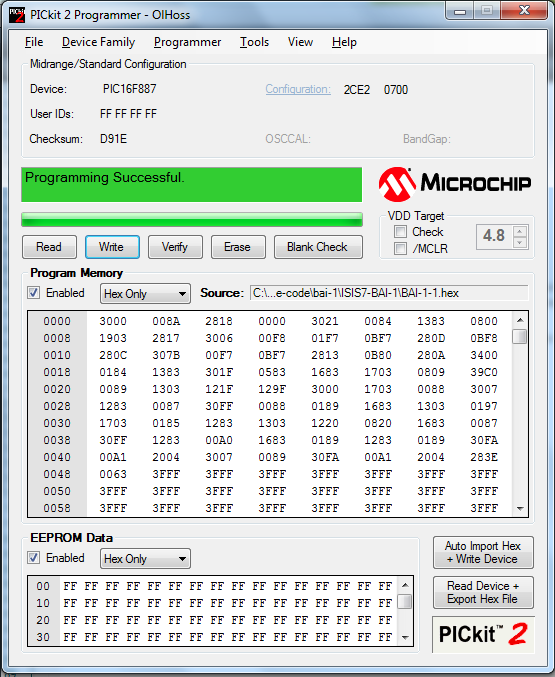
\includegraphics[scale=.5]{phu-luc/image/pickit-22}
\end{center}
\caption{Giao diện khi nạp thành công chương trình cho PIC}
\label{Fig:PICKIT-2-1}
\end{figure}

Ngoài ra cũng cần lưu ý ô điện áp \verb|VDD Target| thông thường từ $4.7V - 5V$.